\documentclass[tikz, margin=3.14mm]{standalone}

\usepackage{tikz}
\usetikzlibrary{decorations, calc, arrows, arrows.meta, positioning}

\begin{document}
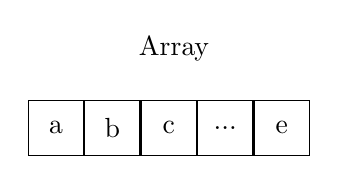
\begin{tikzpicture}[
    array/.style={rectangle, draw, inner sep=5pt, text=black,
        minimum width = 20pt, minimum height = 20pt}
]

    % Nodes ------------------------------------------------------

    \node (title) at (1.5,1) {Array};
    \node[array] (n1) {a};
    \node[array, right=0cm of n1] (n2) {b};
    \node[array, right=0cm of n2] (n3) {c};
    \node[array, right=0cm of n3, minimum width = 20pt] (n4) {...};
    \node[array, right=0cm of n4] (n5) {e};

\end{tikzpicture}
\end{document}